\documentclass[9pt,aspectratio=169,xcolor=table]{beamer}

\usepackage[sfdefault]{roboto}
\usepackage[utf8]{inputenc}
\usepackage[T1]{fontenc}

\usepackage{styles/fluxmacros}
\usefolder{styles}
\usetheme[style=red]{flux}

\definecolor{primaryLight}{HTML}{9B2242}
\definecolor{primary}{HTML}{7B1E3A}
\definecolor{secondary}{HTML}{3A5A6B}
\definecolor{tertiary}{HTML}{8C6A3F}

\usepackage{booktabs}
\usepackage{colortbl}
\usepackage{ragged2e}
\usepackage{amssymb}
\usepackage{multirow}
\usepackage{tikz}
\usetikzlibrary{arrows.meta, positioning, fit, backgrounds, calc, shapes.geometric}
\setbeamertemplate{itemize items}[square]
\usepackage[scaled=.92]{beramono}
\usepackage{listings}
\usepackage{array}
\usepackage{pgfplots}
\pgfplotsset{compat=1.17}
\definecolor{stripe}{gray}{0.94}
\newcommand{\striped}{\rowcolors{1}{white}{stripe}}

\definecolor{codebg}{HTML}{FBF2F4}
\definecolor{codegreen}{rgb}{0,0.45,0}
\definecolor{codestring}{rgb}{0.58,0.1,0.2}
\lstdefinestyle{skpython}{
    basicstyle=\ttfamily\footnotesize,
    keywordstyle=\color{primary}\bfseries,
    commentstyle=\itshape\color{codegreen},
    stringstyle=\ttfamily\color{codestring},
    backgroundcolor=\color{codebg},
    breaklines=true,
    keepspaces=true,
    showspaces=false,
    showstringspaces=false,
    frame=single,
    rulecolor=\color{primary!40},
    numbers=none,
}
\lstdefinestyle{skoutput}{
    basicstyle=\ttfamily\footnotesize,
    backgroundcolor=\color{secondary!8},
    breaklines=true,
    keepspaces=true,
    showspaces=false,
    showstringspaces=false,
    frame=single,
    rulecolor=\color{secondary!50},
    numbers=none,
}
\lstset{language=Python, style=skpython}

\definecolor{cycfill}{HTML}{F3DCE4}
\definecolor{cycline}{HTML}{7B1E3A}
\definecolor{cycdofill}{HTML}{E8EEF0}
\definecolor{cycdoline}{HTML}{3A5A6B}
\tikzset{
  cycstep/.style = {font=\sffamily\small, align=center, rounded corners=2pt,
                     draw=cycline, fill=cycfill, line width=0.7pt,
                     minimum height=7mm, minimum width=20mm, inner sep=3pt},
  cycdo/.style   = {cycstep, fill=cycdofill, draw=cycdoline},
  flow/.style    = {-{Stealth[length=2mm]}, thick, draw=cycline},
}

\AtBeginSection[]
{
{
    \setbeamercolor{background canvas}{bg=primaryLight!6}
    \begin{frame}[plain]
        \frametitle{Table of Contents}
        \tableofcontents[currentsection]
    \end{frame}
}
}

\title{Data Visualization}
\subtitle{\emph{Engineering Computation with Python} --- Chapter 7}
\author{Mun\'{i}m Zabidi}
\institute{\color{primary}Faculty of Electrical Engineering, Universiti Teknologi Malaysia}
\date{\today}
\titlegraphic{assets/logoutmwhite.png}

\begin{document}

\titlepage

\begin{frame}{Table of Contents}
    \tableofcontents
\end{frame}

%===============================================================================
\section{Why Visualize Data?}
%===============================================================================

\begin{frame}{A Formula Tells You What. A Graph Tells You How.}
    \leavevmode
    \begin{block}{Data visualization}
        Turning numbers into pictures that can be reasoned about --- this
        is where engineering mathematics becomes \alert{visible}, and
        among the most practical skills in this course.
    \end{block}

    \vspace{3mm}
    \begin{itemize}\small
        \item A graph summarizes huge amounts of information into one
              picture.
        \item A graph makes it easy to compare multiple sets of measured
              data.
        \item A graph shows directly how one quantity changes in
              response to another.
    \end{itemize}
\end{frame}

\begin{frame}{Every Measurement Has Two Vectors}
    \leavevmode
    Recording scientific data always involves at least two vectors:

    \vspace{2mm}
    \begin{columns}[t]
        \begin{column}{.5\textwidth}
            \begin{block}{Measured variable}
                \small The quantity being observed (plotted on the
                \alert{y-axis}).
            \end{block}
        \end{column}
        \begin{column}{.5\textwidth}
            \begin{block}{Function variable}
                \small The quantity the measurement depends on --- time,
                angle, distance (plotted on the \alert{x-axis}).
            \end{block}
        \end{column}
    \end{columns}

    \vspace{3mm}
    {\small Example: $V(t)$ is a voltage \emph{reading} (measured
    variable) over \emph{time} (function variable). Both vectors must
    have the \alert{same length}.}
\end{frame}

%===============================================================================
\section{2-D Line Plots}
%===============================================================================

\begin{frame}[fragile]{The plot Function}
    \leavevmode
    \texttt{matplotlib.pyplot} makes Matplotlib work like MATLAB. Each
    \texttt{pyplot} function changes a figure in some way:

\begin{lstlisting}
import matplotlib.pyplot as plt
plt.plot([1, 2, 3, 4])
plt.ylabel('some numbers')
plt.show()
\end{lstlisting}

    \vspace{2mm}
    {\small This is the simplest possible plot --- one array, default
    styling, no axis labels on the x-axis.}
\end{frame}

\begin{frame}[fragile]{Example: Plotting a Function}
    \leavevmode
    Plot $y = e^{x/2}$ for $x = 1, \ldots, 10$:

\begin{lstlisting}
import numpy as np
import matplotlib.pyplot as plt

x = np.arange(1, 11)
y = np.exp(x / 2)
plt.plot(x, y)
plt.xlabel('x')
plt.ylabel('exp(x/2)')
plt.title('Exponential Plot')
plt.show()
\end{lstlisting}

    \vspace{1mm}
    {\small Result: a smooth curve rising steeply --- $e^{x/2}$ grows
    faster and faster as $x$ increases.}
\end{frame}

\begin{frame}{Line and Marker Styles}
    \leavevmode
    \small
    A compact format string combines color, marker, and line style ---
    e.g. \texttt{'-mo'} for a solid magenta line with circle markers.

    \vspace{2mm}
    \begin{columns}[t]
        \begin{column}{.5\textwidth}
            \striped
            \begin{center}
            \begin{tabular}{cl}
                \toprule
                \textbf{Spec} & \textbf{Style} \\
                \midrule
                \texttt{'-'}  & solid \\
                \texttt{':'}  & dotted \\
                \texttt{'--'} & dashed \\
                \texttt{'-.'} & dash-dot \\
                \bottomrule
            \end{tabular}
            \end{center}
        \end{column}
        \begin{column}{.5\textwidth}
            \small Common markers: \texttt{'.'} point, \texttt{'o'}
            circle, \texttt{'s'} square, \texttt{'\^{}'} triangle,
            \texttt{'*'} star.

            \vspace{2mm}
            Colors: \texttt{b}, \texttt{g}, \texttt{r}, \texttt{c},
            \texttt{m}, \texttt{y}, \texttt{k}, \texttt{w}.
        \end{column}
    \end{columns}
\end{frame}

\begin{frame}[fragile]{Example: A Styled Sine Wave}
    \leavevmode
\begin{lstlisting}
x = np.arange(1, 501, 10)
y = np.sin(5 * x)
plt.plot(x, y, '-mo')   # magenta line, circle markers
plt.xlabel('x')
plt.ylabel('sin(5x)')
plt.title('Sine Wave Plot')
plt.show()
\end{lstlisting}

    \vspace{2mm}
    {\small Result: an oscillating curve, each sample point marked with
    a magenta circle, connected by a solid magenta line.}
\end{frame}

%===============================================================================
\section{Plot Formatting}
%===============================================================================

\begin{frame}{Decorating a Plot}
    \leavevmode
    \small
    \striped
    \begin{center}
    \begin{tabular}{p{4.0cm}p{5.0cm}}
        \toprule
        \textbf{Properties} & \textbf{Function} \\
        \midrule
        Title, axis labels, legend & \texttt{title}, \texttt{xlabel},
        \texttt{ylabel}, \texttt{legend} \\
        Axis limits & \texttt{xlim}, \texttt{ylim}, \texttt{axis} \\
        Grid and ticks & \texttt{grid}, \texttt{xticks}, \texttt{yticks} \\
        Multiple plots & \texttt{figure}, \texttt{subplot} \\
        \bottomrule
    \end{tabular}
    \end{center}

    \vspace{3mm}
    \begin{alertblock}{A plot is not complete just because it displays}
        It needs axis labels with \alert{units}, a title, and a legend
        when more than one curve is shown.
    \end{alertblock}
\end{frame}

\begin{frame}[fragile]{LaTeX Math Symbols in Plot Labels}
    \leavevmode
    Matplotlib renders LaTeX-style math inside a \alert{raw string}
    between \texttt{\$} symbols:

\begin{lstlisting}
plt.xlabel(r'$\omega$')
plt.title(r'Sin($\omega$) Graph')
\end{lstlisting}

    \vspace{2mm}
    \begin{block}{Note the leading r}
        \texttt{r'...'} is a raw string, needed so Python does not try
        to interpret the backslash. This is matplotlib's own mathtext
        renderer, not a full LaTeX engine.
    \end{block}
\end{frame}

\begin{frame}[fragile]{Example: Custom Tick Labels}
    \leavevmode
    Plot $\sin(\omega)$ with ticks expressed as multiples of $\pi$:

\begin{lstlisting}
w = np.linspace(0, 2*np.pi, 1000)
y = np.sin(w)
ticks = [0, 0.5*np.pi, np.pi, 1.5*np.pi, 2*np.pi]
labels = ["0", r"$0.5\pi$", r"$\pi$", r"$1.5\pi$", r"$2\pi$"]

plt.plot(w, y)
plt.xticks(ticks, labels)
plt.grid(True)
plt.show()
\end{lstlisting}
\end{frame}

\begin{frame}[fragile]{Multiple Curves on One Graph}
    \leavevmode
    Call \texttt{plt.plot} repeatedly before \texttt{plt.show()}; each
    call gets its own style and label.

\begin{lstlisting}
x = np.arange(-10, 10.5, 0.5)
f = 3*x**4 + 2*x**3 + 7*x + 9
g = 5*x**3 + 9*x + 2

plt.plot(x, f, '-xm', label='f(x)')
plt.plot(x, g, '--ok', label='g(x)')
plt.legend()
plt.show()
\end{lstlisting}

    \vspace{1mm}
    {\small Result: two curves on shared axes, one magenta with
    x-markers, one black dashed with circles --- their intersection
    points are visible directly.}
\end{frame}

%===============================================================================
\section{Subplots}
%===============================================================================

\begin{frame}[fragile]{The subplot Function}
    \leavevmode
    An array of plots within one figure --- each is a \alert{subplot}:

\begin{lstlisting}
plt.subplot(m, n, p)
\end{lstlisting}

    \vspace{2mm}
    \begin{itemize}
        \item $m$, $n$: grid size (rows, columns)
        \item $p$: position, numbered \alert{left to right, then top to
              bottom} --- the opposite convention to array indexing
    \end{itemize}
\end{frame}

\begin{frame}[fragile]{Example: Stacked Subplots}
    \leavevmode
\begin{lstlisting}
x = np.linspace(0, 10, 100)
y = np.cos(3 * x)
z = np.sin(x)

plt.subplot(2, 1, 1)
plt.plot(x, y)
plt.title('y = cos(3x)')

plt.subplot(2, 1, 2)
plt.plot(x, z)
plt.title('z = sin(x)')

plt.tight_layout()   # adjusts subplots to avoid overlap
plt.show()
\end{lstlisting}
\end{frame}

\begin{frame}{The RC Low-Pass Filter}
    \leavevmode
    \begin{columns}[t]
        \begin{column}{.55\textwidth}
            $R$ and $C$ form a voltage divider; the output is taken
            across the capacitor.

            \vspace{2mm}
            \[
            H = \frac{1}{1 + j 2\pi f RC}
            \]
            \[
            |H| = \frac{1}{\sqrt{1+(2\pi fRC)^2}}, \;\; \angle H = -\tan^{-1}(2\pi fRC)
            \]
        \end{column}
        \begin{column}{.4\textwidth}
            \begin{center}
            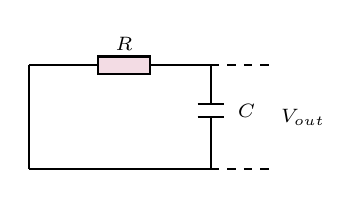
\begin{tikzpicture}[scale=0.55, every node/.style={font=\scriptsize}]
                \draw[thick] (0,0) -- (0,2.4);
                \draw[thick] (0,2.4) -- (1.6,2.4);
                \draw[thick,fill=cycfill] (1.6,2.2) rectangle (2.8,2.6);
                \node at (2.2,2.9) {$R$};
                \draw[thick] (2.8,2.4) -- (4.2,2.4);
                \draw[thick] (4.2,2.4) -- (4.2,1.5);
                \draw[thick] (3.9,1.5) -- (4.5,1.5);
                \draw[thick] (3.9,1.2) -- (4.5,1.2);
                \node[right] at (4.6,1.35) {$C$};
                \draw[thick] (4.2,1.2) -- (4.2,0) -- (0,0);
                \draw[thick,dashed] (4.2,2.4) -- (5.6,2.4);
                \draw[thick,dashed] (4.2,0) -- (5.6,0);
                \node[right] at (5.6,1.2) {$V_{out}$};
            \end{tikzpicture}
            \end{center}
        \end{column}
    \end{columns}

    \vspace{2mm}
    {\small Since capacitor impedance falls as frequency rises, less
    input reaches the output at high frequency --- a \alert{low-pass}
    filter.}
\end{frame}

\begin{frame}[fragile]{Magnitude and Phase of the RC Filter}
    \leavevmode
\begin{lstlisting}
C, R = 0.47e-6, 4.7e3
f = np.linspace(0, 10000, 10000)

H = 1 / (1 + 1j * 2 * np.pi * f * R * C)
Magnitude = np.abs(H)
Phase = np.angle(H)

plt.subplot(2, 1, 1)
plt.plot(f / 1000, Magnitude)
plt.xlabel('Frequency (kHz)')

plt.subplot(2, 1, 2)
plt.plot(f / 1000, Phase / np.pi)
plt.ylabel(r'Phase ($\pi$ rad)')
\end{lstlisting}

    \vspace{1mm}
    {\small \texttt{np.abs(H)} and \texttt{np.angle(H)} give magnitude
    and phase automatically from a complex transfer function.}
\end{frame}

\begin{frame}[fragile]{Quadrant Subplots: A 2-by-2 Grid}
    \leavevmode
    Plot four sinusoids of different frequencies in one figure:

\begin{lstlisting}
t = np.arange(0, 1.001, 0.001)
for F in range(1, 5):
    y = np.sin(2 * np.pi * F * t)
    plt.subplot(2, 2, F)
    plt.plot(t, y)
    plt.title(f'{F} Cycle')

plt.tight_layout()
plt.show()
\end{lstlisting}

    \vspace{1mm}
    {\small Result: four small plots in a 2$\times$2 grid, each showing
    one more oscillation than the last.}
\end{frame}

%===============================================================================
\section{Specialized Plots}
%===============================================================================

\begin{frame}[fragile]{Stem Plot: Discrete Signals}
    \leavevmode
    \texttt{plt.stem} draws a marker at each sample connected to a
    baseline --- for \alert{discrete-time} signals, not continuous ones:

\begin{lstlisting}
n = np.arange(0, 101)
w = 0.04 * np.pi
y = np.sin(w * n)

plt.stem(n, y)
plt.xlabel('sample, n')
plt.ylabel(r'sin($\omega n$)')
plt.show()
\end{lstlisting}

    \vspace{1mm}
    {\small Each of the 101 samples is drawn as a separate marker on a
    vertical stem, not joined by a continuous line.}
\end{frame}

\begin{frame}{Logarithmic Scales}
    \leavevmode
    A nonlinear scale for data spanning a \alert{large range} of
    magnitudes:

    \vspace{2mm}
    \begin{itemize}
        \item Earthquake strength (Richter), sound loudness (decibel),
              pH, frequency range (Bode plot)
    \end{itemize}

    \vspace{3mm}
    \begin{columns}[t]
        \begin{column}{.33\textwidth}
            \begin{block}{\scriptsize semilogx}
                \scriptsize x-axis log
            \end{block}
        \end{column}
        \begin{column}{.33\textwidth}
            \begin{block}{\scriptsize semilogy}
                \scriptsize y-axis log
            \end{block}
        \end{column}
        \begin{column}{.33\textwidth}
            \begin{block}{\scriptsize loglog}
                \scriptsize both axes log
            \end{block}
        \end{column}
    \end{columns}
\end{frame}

\begin{frame}[fragile]{Example: Loudness, Linear vs. Log}
    \leavevmode
    Loudness spans library ($\sim\!10^2\,\text{W}$) to a rock concert
    ($\sim\!10^{11}\,\text{W}$):

\begin{lstlisting}
L = [7.94e2, 1.26e6, 3.16e8, 1.58e9, 6.3e9, 1.99e11]

plt.subplot(2, 1, 1)
plt.plot(L, '-bo')          # linear: small values near zero, invisible
plt.subplot(2, 1, 2)
plt.semilogy(L, '-bo')      # log: all six values spread out clearly
\end{lstlisting}

    \vspace{1mm}
    \begin{alertblock}{Why it matters}
        On the linear plot, the four smallest values are visually
        indistinguishable near zero. The log plot reveals detail across
        the \alert{entire} range.
    \end{alertblock}
\end{frame}

\begin{frame}{The Bode Plot}
    \leavevmode
    A \alert{Bode plot} shows how a system responds across frequency ---
    the standard tool for filters, amplifiers, control systems.

    \vspace{2mm}
    \begin{columns}[t]
        \begin{column}{.5\textwidth}
            \begin{block}{Magnitude}
                \small How much the output is scaled, in
                \alert{decibels}: $20\log_{10}|H|$.
            \end{block}
        \end{column}
        \begin{column}{.5\textwidth}
            \begin{block}{Phase}
                \small How far the output is shifted in time, in
                degrees.
            \end{block}
        \end{column}
    \end{columns}

    \vspace{3mm}
    {\small Two stacked plots sharing one \alert{logarithmic frequency
    axis}.}
\end{frame}

\begin{frame}[fragile]{Generating the Frequency Axis: logspace, Not linspace}
    \leavevmode
    Because the frequency axis is logarithmic, frequencies must be
    generated with \texttt{np.logspace}:

\begin{lstlisting}
R, C = 4.7e3, 0.47e-6
fc = 1 / (2 * np.pi * R * C)   # cutoff, about 72 Hz

f = np.logspace(0, 4, 500)     # 1 Hz to 10 kHz, log-spaced
H = 1 / (1 + 1j * 2 * np.pi * f * R * C)
magnitude_db = 20 * np.log10(np.abs(H))
phase_deg = np.degrees(np.angle(H))
\end{lstlisting}

    \vspace{1mm}
    \begin{alertblock}{Why it matters}
        A \alert{linear} range of $10{,}000$ points would place only 9
        below $10\,\text{Hz}$ and crowd $9{,}000$ above $1\,\text{kHz}$
        --- barely sampling the bend, the part worth seeing.
    \end{alertblock}
\end{frame}

\begin{frame}{Reading the Bode Plot}
    \leavevmode
    \small
    \begin{columns}[t]
        \begin{column}{.45\textwidth}
            \begin{center}
            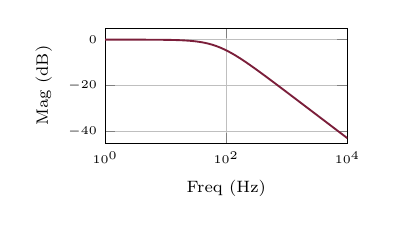
\begin{tikzpicture}[scale=0.85]
                \begin{axis}[
                    width=5.2cm, height=3.3cm,
                    xmode=log, xmin=1, xmax=10000,
                    ymin=-45, ymax=5,
                    xlabel={\scriptsize Freq (Hz)},
                    ylabel={\scriptsize Mag (dB)},
                    label style={font=\tiny},
                    tick label style={font=\tiny},
                    grid=both,
                ]
                \addplot[primary, thick, domain=1:10000, samples=60]
                    {-10*log10(1+(x/72.1)^2)};
                \end{axis}
            \end{tikzpicture}
            \end{center}
        \end{column}
        \begin{column}{.55\textwidth}
            \begin{itemize}
                \item \textbf{Flat passband.} Below $\sim\!20\,\text{Hz}$,
                      magnitude sits at $0\,\text{dB}$.
                \item \textbf{Cutoff} $f_c \approx 72\,\text{Hz}$: magnitude
                      falls to $-3\,\text{dB}$, phase is $-45^\circ$.
                \item \textbf{Roll-off.} Above cutoff, $-20\,\text{dB}$ per
                      decade.
            \end{itemize}
        \end{column}
    \end{columns}

    \vspace{2mm}
    {\small This is exactly how unwanted high-frequency noise is removed
    from a measured signal.}
\end{frame}

%===============================================================================
\section{Statistical Plots}
%===============================================================================

\begin{frame}[fragile]{Histogram: Shape of a Dataset}
    \leavevmode
\begin{lstlisting}
data = np.random.randn(1000)
plt.hist(data, bins=50)
plt.xlabel('Data Value')
plt.ylabel('Frequency')
plt.show()
\end{lstlisting}

    \vspace{2mm}
    \begin{block}{What a histogram reveals}
        Central tendency, spread, and shape of a dataset --- useful for
        spotting outliers, a standard tool in Exploratory Data Analysis.
    \end{block}
\end{frame}

\begin{frame}[fragile]{Box Plots: Median, Quartiles, Outliers}
    \leavevmode
\begin{lstlisting}
plt.boxplot(data)
plt.ylabel('Value')
plt.show()
\end{lstlisting}

    \vspace{2mm}
    \begin{block}{What the box shows}
        The box spans the interquartile range (25th to 75th percentile),
        the line inside is the \alert{median}, and points beyond the
        whiskers are flagged as potential \alert{outliers}.
    \end{block}

    \vspace{1mm}
    {\small Variants exist for grouped, notched, and horizontal
    comparisons --- the IQR rule behind this returns in Chapter 11.}
\end{frame}

%===============================================================================
\section{The Bench Experiment}
%===============================================================================

\begin{frame}[fragile]{Plotting the Recurring Dataset}
    \leavevmode
    101 rows --- far too many to read as numbers, exactly right to see
    at a glance as a picture:

\begin{lstlisting}
import pandas as pd
data = pd.read_csv('bench_rc.csv')
t = data['time_s']
v = data['voltage_V']

plt.plot(t, v, 'o-', markersize=3, label='Measured $v(t)$')
plt.xlabel('Time (s)')
plt.ylabel('Capacitor voltage (V)')
plt.grid(True, linestyle='--', alpha=0.6)
plt.legend()
plt.show()
\end{lstlisting}
\end{frame}

\begin{frame}{Engineering Sanity Checks}
    \leavevmode
    \small
    A plot should always be checked before you trust it:

    \vspace{2mm}
    \begin{itemize}
        \item \textbf{Units.} Axis runs $0$--$12\,\text{V}$, matching
              the $12\,\text{V}$ supply.
        \item \textbf{Magnitude.} Starts at $12\,\text{V}$, decays
              toward zero --- as a discharging capacitor must.
        \item \textbf{Limiting case.} At $t=\tau=0.47\,\text{s}$,
              voltage should be $e^{-1}\approx 37\%$ of $12\,\text{V}
              \approx 4.4\,\text{V}$. The graph agrees.
        \item \textbf{Independent check.} $i = v/R$ at $t=0$ gives
              $2.55\,\text{mA}$, matching the recorded current.
    \end{itemize}

    \vspace{2mm}
    \begin{alertblock}{What the plot reveals that numbers would not}
        A visible break near $t=0.8\,\text{s}$ --- three dropped
        samples. Chapter 11 shows how to fix this kind of gap.
    \end{alertblock}
\end{frame}

%===============================================================================
\section{Preview: Slope}
%===============================================================================

\begin{frame}{The Slope of a Curve}
    \leavevmode
    Chapter 6 previewed \alert{accumulation}. Plotting makes its
    counterpart just as visible: the \alert{slope} --- different at
    every point along a curve.

    \vspace{2mm}
    \[
    \text{slope} = \frac{\Delta y}{\Delta x} = \frac{y_2-y_1}{x_2-x_1}
    \]

    \vspace{2mm}
    For $y=x^2$: gentle rise between $x=0$ and $x=1$, steep rise between
    $x=3$ and $x=4$ --- same curve, very different local slope.
\end{frame}

\begin{frame}[fragile]{Measuring Slope Over Two Intervals}
    \leavevmode
\begin{lstlisting}
x = np.linspace(0, 4, 100)
y = x**2

for x1, x2 in [(0, 1), (3, 4)]:
    slope = (x2**2 - x1**2) / (x2 - x1)
    print(f"Slope {x1} to {x2}: {slope}")
\end{lstlisting}
\begin{lstlisting}[style=skoutput]
Slope 0 to 1: 1.0
Slope 3 to 4: 7.0
\end{lstlisting}

    \vspace{1mm}
    \begin{alertblock}{Slope is almost always a rate}
        Charge vs. time $\to$ slope is current. Position vs. time $\to$
        slope is velocity. Shrinking the interval to a point is exactly
        what a \alert{derivative} does (Chapter 13).
    \end{alertblock}
\end{frame}

%===============================================================================
\section{Summary}
%===============================================================================

\begin{frame}{What You Should Take Away}
    \leavevmode
    \small
    \begin{itemize}
        \item \texttt{plt.plot()} draws a 2-D line plot; it needs axis
              labels with \textbf{units}, a title, and a legend for
              multiple curves.
        \item \texttt{plt.subplot()} arranges several plots in a grid
              --- how related quantities are compared on a common axis.
        \item \textbf{Logarithmic axes} turn exponential and power-law
              relationships into straight lines.
        \item A \textbf{Bode plot} shows magnitude (dB) and phase
              against log frequency; generate frequencies with
              \texttt{np.logspace}, not \texttt{np.linspace}.
    \end{itemize}
\end{frame}

\begin{frame}{What You Should Take Away (continued)}
    \leavevmode
    \small
    \begin{itemize}
        \item \textbf{Histograms} and \textbf{box plots} reveal a
              dataset's shape, spread, and outliers.
        \item Always run \textbf{engineering sanity checks} on a plot:
              units, magnitude, limiting cases, independent checks.
        \item The \textbf{slope} of a curve is a rate --- shrinking the
              interval to a point gives the derivative.
    \end{itemize}

    \vspace{4mm}
    \begin{center}
        \large\color{primary}\textbf{Next: Complex Numbers and AC Circuits}
    \end{center}
\end{frame}

\end{document}
